\section{The Orienteering Problem}

\begin{frame}{The Orienteering Problem}

	\note[item]{
		Proper definition of the OP \begin{itemize}
			\item Start with an undirected graph
		\end{itemize}
	}
	\note[item] {
		Profit function $s$ for the nodes \begin{itemize}
			\item Also called \enquote{score}
		\end{itemize}
	}
	\note[item]{
		Cost function $t$ for the edges \begin{itemize}
			\item Also \enquote{distance}, \enquote{travel time}, \enquote{weight}
		\end{itemize}
	}
	\note[item]{
		Maximum cost $T_{max}$
	}
	\note[item]{
		Orienteering Problem \begin{itemize}
			\item Want a path from $v_1$ to $v_n$ \begin{itemize}
				      \item Need not be fixed but often are
				      \item Named like this for convenience
			      \end{itemize}
			\item Path should maximize the total profit...
			\item ...while respecting the cost limit $T_{max}$
		\end{itemize}
	}

	\begin{definition}[Orienteering Problem \cite{vansteenwegen_orienteering_2011}]
		\begin{itemize}
			\item Graph $G=(V = \{v_1, \dots, v_n\}, E)$
			\item Score function $s: V \rightarrow \mathbb{R}_+$
			\item Cost function $t: E \rightarrow \mathbb{R}_+$
			\item Cost Limit $T_{max} \in \mathbb{R}_+$
			\item [$\Rightarrow$] Find path $P$ with maximal profit and cost less than $T_{max}$
		\end{itemize}
	\end{definition}

\end{frame}

\begin{frame}{Example}

	\note<1>[item]{
		Example OP instance \begin{itemize}
			\item $T_{max} = 6$
			\item Edges between all nodes (omitted for clarity)
			\item Horizontal/Vertical distance between neighboring nodes: 1
			\item Diagonal movement: $\sqrt 2 \approx 1.4$
		\end{itemize}}
	\note<1>[item]{Ask audience: What is the optimal path?}
	\note<2>[item]{Best path as far as I can see}

	\centering
	\begin{columns}
		\begin{column}{0.48\textwidth}
			\begin{itemize}
				\item<1-> Grid spacing of $1$
				\item<1-> $T_{max} = 6$
				\item<2> $T(P) = 4 + \sqrt 2 < 6$
				\item<2> $S(P) = 28$
			\end{itemize}
		\end{column}
		\begin{column}{0.48\textwidth}
			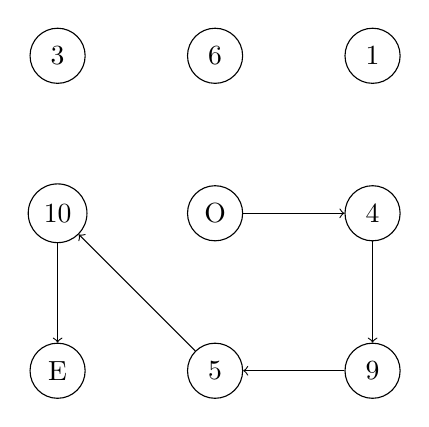
\begin{tikzpicture}[every node/.style={draw,shape=circle,minimum size=7mm}]
				\node (origin) at (0,0) {O};
				\node (1) at (-2,0) {10};
				\node (2) at (-2,2) {3};
				\node (3) at (0,2) {6};
				\node (4) at (2,0) {4};
				\node (5) at (0,-2) {5};
				\node (6) at (2,-2) {9};
				\node (7) at (2,2) {1};
				\node (end) at (-2,-2) {E};

				\draw<2>[->] (origin) -- (4);
				\draw<2>[->] (4) -- (6);
				\draw<2>[->] (6) -- (5);
				\draw<2>[->] (5) -- (1);
				\draw<2>[->] (1) -- (end);
			\end{tikzpicture}
		\end{column}
	\end{columns}
\end{frame}

\begin{frame}{Complete Graphs}

	\note<1>[item]{
		Getting into the problem \begin{itemize}
			\item Restrictions on allowed input graphs
			\item Introduce common ones in order of strictness
			\item After: introduce algorithms and try to reduce the restrictions they require
		\end{itemize}
	}
	\note<2->[item]{First: Complete Graph}
	\note<2->[item]{
		Probably known to everyone \begin{itemize}
			\item But for completeness' sake
		\end{itemize}
	}
	\note<2->[item]{
		Almost unanimous
	}
	\note<2->[item]{
		Simple to transform any graph into complete graph. Insert missing edges with weight \begin{itemize}
			\item Weight of the shortest path between nodes
			\item $\infty$ if the missing edges should not be taken \begin{itemize}
				      \item Might not work for all algorithms though (example later)
			      \end{itemize}
		\end{itemize}
	}

	\begin{columns}
		\begin{column}{0.58\textwidth}
			\only<2->{
				\begin{definition}[Complete Graphs]
					\begin{itemize}
						\item Edge exists between all nodes
					\end{itemize}
				\end{definition}
			}

			\only<2->{ Almost unanimous in the literature \cite{vansteenwegen_orienteering_2011,laporte_selective_1990,santini_hazardous_2022,szwarc_novel_2022}}
		\end{column}
		\begin{column}{0.4\textwidth}
			\only<2->{
				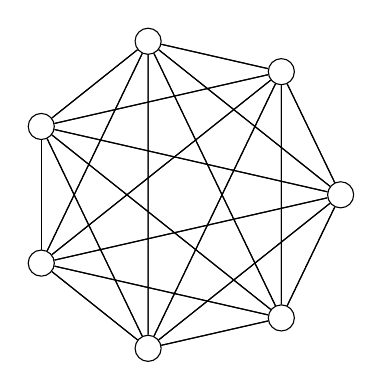
\begin{tikzpicture}
					\foreach \a in {1,2,...,7} {
							\draw (\a*360/7: 2cm) node[shape=circle,draw] (\a) {};
						}
					\foreach \a in {1,2,...,7} {
							\foreach \b in {1,2,...,7} {
									\draw (\a) -- (\b);
								}
						}
				\end{tikzpicture}
			}
		\end{column}
	\end{columns}
\end{frame}

\begin{frame}{Triangle Inequality}
	\note<1->[item]{
		First actual restriction \begin{itemize}
			\item Similarly defined as in geometry
		\end{itemize}
	}
	\note<1->[item]{
		Any three nodes' weights satisfy the triangle inequality
	}
	\note<2->[item]{
		$\Rightarrow$ The direct edge is always the shortest path between nodes. \begin{itemize}
			\item No detour will ever be faster
		\end{itemize}
	}

	\only<1->{
		\begin{definition}[Triangle Inequality \cite{black_triangle_2004}]
			\begin{itemize}
				\item Complete Graph
				\item For all nodes $t(u,w) \leq t(u,v) + t(u,v)$
			\end{itemize}
		\end{definition}
	}

	\begin{itemize}
		\item<2->[$\Rightarrow$] No shorter path than the direct edge
	\end{itemize}
\end{frame}

\begin{frame}{Euclidean Graphs}
	\note<1->{Definition like in geometry}
	\note<1->{
		Nodes are points in the euclidean plane \begin{itemize}
			\item Edge weights are distances between them
		\end{itemize}
	}
	\note<1->{
		Note, that this entails completeness and the triangle inequality \begin{itemize}
			\item[$\Rightarrow$] Entails the previous two restrictions
		\end{itemize}
	}
	\note<2->{Commonly seen in the literature}

	\begin{definition}[Euclidean Graphs]
		\begin{itemize}
			\item<1-> Coordinates $(x_i, y_i)^\intercal \in \mathbb{R}^2$
			\item<1-> Edge weights $t(v_i,v_j) := \sqrt{(x_i - x_j)^2 + (y_i - y_j)^2}$
		\end{itemize}
	\end{definition}

	\only<2->{ Very common in the literature \cite{geem_harmony_2005,golden_orienteering_1987,szwarc_novel_2022,tsiligiridis_heuristic_1984}}
\end{frame}